\section{Attitude Reference}

The main attitude controllers require an attitude reference quaternion and a reference angular velocity to track. In the simulation environment, the attitude reference quaternion is given in orbit frame, the angular velocity reference in ECI frame. As discussed above, two attitude control goals are distinguished: nadir pointing and Earth station tracking. For nadir pointing, the attitude reference quaternion is simply assigned as $[0 \ 0 \ 0 \ 1]^T$ and the angular velocity reference is identical to the orbit angular velocity. Creating the references for Earth station tracking are not as trivial.

For Earth station tracking, the reference quaternion can be calculated using the positions of the satellite, the station, and the center of Earth. The unit rotation axis of the attitude quaternion is $\vec{e} = \frac{^{sat}\vec{R}_{o} \times ^{sat}\vec{R}_{st}}{||^{sat}\vec{R}_{o} \times ^{sat}\vec{R}_{st}||}$, where ${^{sat}\vec{R}_{o}}$ is the distance from center of Earth to the satellite and $^{sat}\vec{R}_{st}$ is the distance from station to the satellite. 

The angle between the nadir pointing and the station pointing vectors can be calculated using the law of cosines. The attitude quaternion in orbit frame is calculated using the quaternion rotation formula $ \vec q = e^{\frac{\Phi}{2} (e_1 \textbf{i}+ e_2 \textbf{j} + e_3 \textbf{k} + e_4)} = \cos \frac{\Phi}{2} + (e_1 \textbf{i}+ e_2 \textbf{j} + e_3 \textbf{k}) \sin \frac{\Phi}{2}$, as described in appendix \ref{chap:A}. The corresponding angular velocity reference can be calculated using the equation described in appendix \ref{eq:finaleq}.



%For the satellite to be able to track a given static position on Earth within 1°, a quaternion is computed. Therefore, this quaternion represents the vector that points from the orbit position to the station.
%
%The tracking quaternion is calculated by giving a quaternion attitude demand in orbit frame and by using this it is possible to calculate the angular velocity demand. The position vector of the station and the position of the satellite are known, then this two are subtracted and results the direction between them which is transformed into a quaternion.
%
%In the simulation the Earth station is stationary which means that it does not move in the inertial frame.
%
%The way it can be verify that the error is around 1°, is by looking at the attitude error quaternion.  The scalar part which represent $\cos (\frac{\alpha}{2}) $ and then calculate $\alpha$ based on that.  That $\alpha$ it should not be bigger then 1°.

\begin{figure}[H]
	\centering
	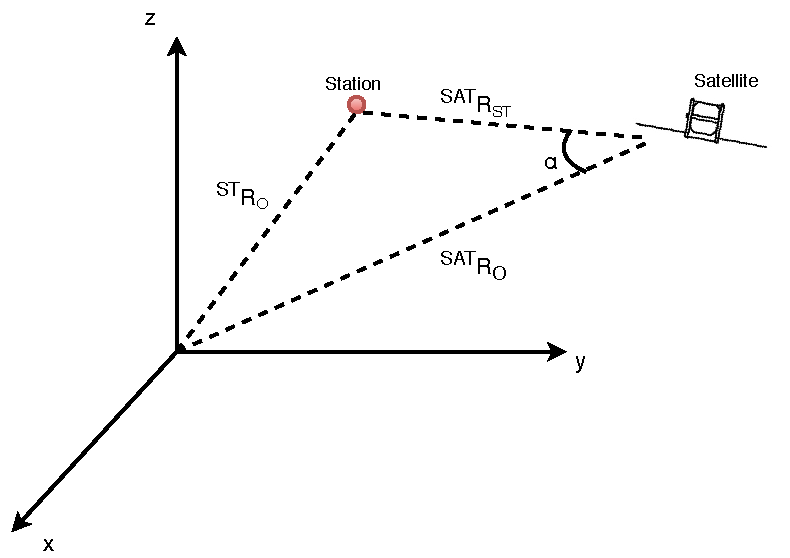
\includegraphics[width=0.7\linewidth]{figures/ST}
	\caption{Tracking a target on Earth }
	\label{fig:TS}
\end{figure}
